\chapter{Dataset}
\label{DatasetChap}

In this chapter we discuss how the dataset was choosen, how we create it, and the different parameters 
acceseable when creating it. 

\section{Background}

Our first decision was in desciding the task our AI was going to solve.
In selecting the task our AI model was going to solve we had a few attributes in mind. We did not want something to complex,
it had to be simple to implement and change,  as we were to make a Proof Of Consept. At the same time the problem should not be too simple,
we want to check if our method will convey the AI models errors with respect to the ground truth.
We also wanted to able to test our system with different AIs. To achive this we wanted our task to achive this we wanted the ground truth
to be easily changeable, so we can compare AIs trained on different ground truths.

In the end we chose the task of predicting an underlaying boolean function given bitmaps contaning a subset of the literals {A,B,C,D}.
Present literals in the bitmap is set to True, and all others are set to False. The label for a given instance is 
then found by calulcateing the underlaying boolean function with literal assigned as descrebied above, giving a label of
1 – being True – or 0 – being False.

This choice fits our demands as we can easily create a new ground truth by swapping the ground truth boolean function. This means our model is not over complex. 
At the same time the bitmaps representation of literals gives us the possibility of huge traing datasets, which has the possibility of creating
more or less complex datasets – different orientations, sizes and letter styles. 

\section{Description of an instance}
\label{InstanceDescription}

In more detail, the input to our AI will be a 64x64 bitmap. The cells in the bitmap will either have the value $0$ or $255$.
The cells having the value $255$ will together make up one or more letter from a predetermined letter set $L = {A,B,C,D}$.
Three examples of the instances are shown below.
 
\begin{figure}[!htb]
    \minipage{0.32\textwidth}
      
\includegraphics[width=\linewidth]{figures/Bitmap-A}
      \caption{Bitmap A}\label{Bitmap-A}
    \endminipage\hfill
    \minipage{0.32\textwidth}
      
\includegraphics[width=\linewidth]{figures/Bitmap-AD}
      \caption{Bitmap AD}
      \label{Bitmap-AD}
    \endminipage\hfill
    \minipage{0.32\textwidth}%
      
\includegraphics[width=\linewidth]{figures/Bitmap-BCD}
      \caption{Bitmap BCD} 
      \label{Bitmap-BCD}
    \endminipage
\end{figure}

% TODO: This seems bad. Maybe fix? Image smaller?
We also have different parameters to active. These will be discussed in \ref{ParametersGenDataset}. 
The images above are of the smallest varience possible. Below are examples showing images 
from our dataset at highest possible varience.

\begin{figure}[!htb]
    \minipage{0.32\textwidth}
      
\includegraphics[width=\linewidth]{figures/Bitmap-highvar-ABCD}
      \caption{Bitmap ABCD}
      \label{Bitmap-highvar-ABCD}
    \endminipage\hfill
    \minipage{0.32\textwidth}
      
\includegraphics[width=\linewidth]{figures/Bitmap-highvar-ABD}
      \caption{Bitmap ABD}
      \label{Bitmap-highvar-ABD}
    \endminipage\hfill
    \minipage{0.32\textwidth}%
      
\includegraphics[width=\linewidth]{figures/Bitmap-highvar-CD}
      \caption{Bitmap CD} 
      \label{Bitmap-highvar-CD}
    \endminipage
\end{figure}


\section{Properties of instance}
We want to have som clear properties for each data instance. These are mostly sanity checks to make sure
our AI will be given decent data. Altough intuitive, its important to make sure our data is sane. 
Bad data in, means bad perdictions comming out. 

Our rules for the data goes as follows:
\begin{itemize}
    \item For each letter, the entirety of the letter is to be contained within the picture. 
    \item No letter is to overlap with another letter. 
    \item The size of the letter should not be to small. The letter shall contain enough pixles, such that the characteristics of the letter is mainteind. E.g. clearly recognizeable for a human.
  \end{itemize}


\section{Parameters generating instances}
\label{ParametersGenDataset}
When generating data we have quite a few differtent parameters, all contributing to more or less complexity
in our data. The goal of having different parameters for dataset generating is to be able to have a smooth increasing 
in difficulty for our AI. Using this we can find a suitable dataset for our AI models, where they preforme resonabley well. 
We can also try to detect different overfittings based on these parameters.

\subsection{$FixedSquares$ – placement of letter}
For the parameter $FixedSquares$ we divide the image into four squares –top left, top right, bottom left, bottom right. 
Each of these square might then contain a letter. Crucially no letter is overlapping these squares.
All of figures \ref{Bitmap-A},  \ref{Bitmap-AD} and \ref{Bitmap-BCD} have $FixedSquares$.
Having this parameter turned on will make the dataset less complex, as its counter part is to just place freely.
Without $FixedSquares$ the algorithm might find all letters at the top of the image or at the bottom, increasing the
varience of the dataset. This corresponds to a more complex dataset, less prone to be easily overfitted.


\subsection{$Rotation$ – orientation of the letter}
With the parameter $Rotation$ we alow the letters to have different orientations. 
We have slected a subset of orientations $O=\{ 0 ^{\circ}, 45^{\circ}, 90^{\circ}, 135^{\circ}, 180^{\circ}, 225^{\circ},270^{\circ},315^{\circ}\}$. 
Letting each letter take on one of these orientations increase varience and complexity in our dataset. 
Below is an example of an image from a dataset with $Rotation$ allowed.
 
\begin{figure}[h]
    \centering
    
\includegraphics[scale=0.2]{figures/Bitmap-rot-ABC}
    \caption{Bitmap w/rotation ABC} 
    \label{Bitmap-rot-ABC}
\end{figure}

\subsection{$Scale$ - size of the letter}
With $Scale$ we allow letters to have different sizes. Importantly no letter can be made to big \ref{Bitmap-big-ACD}, as
it has to fit inside the image. Nor can it be made to small \ref{Bitmap-small-AB}, as it needs to be recognizeable. 

\begin{figure}[!htb]
    \minipage{0.4\textwidth}
      
\includegraphics[width=\linewidth]{figures/Bitmap-big-ACD}
      \caption{Bitmap ACD, too big. Overlapping, and out of image.}
      \label{Bitmap-big-ACD}
    \endminipage\hfill
    \minipage{0.4\textwidth}
      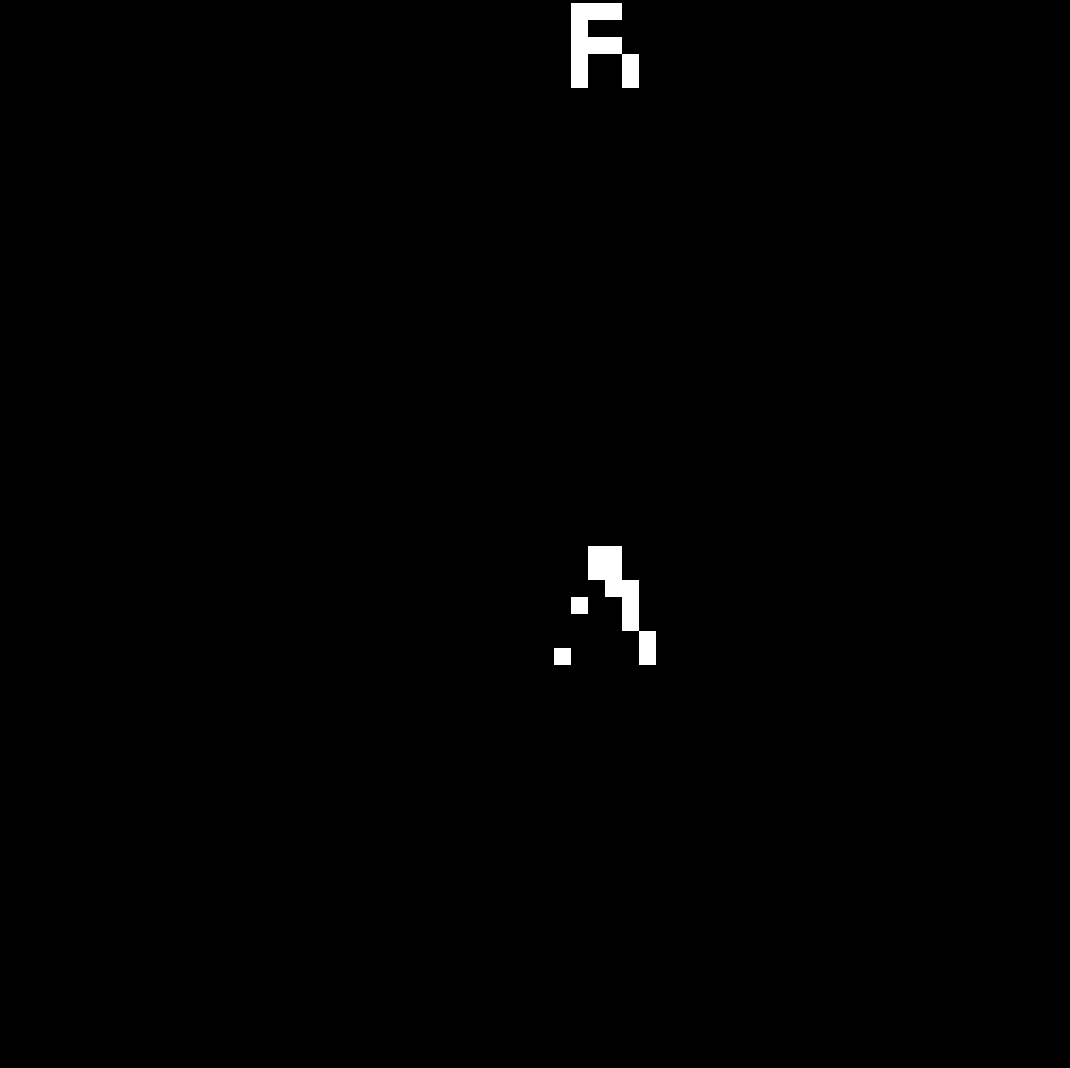
\includegraphics[width=\linewidth]{figures/Bitmap-small-AB}
      \caption{Bitmap AB, too small. A is broken up, B looks like R.} 
      \label{Bitmap-small-AB}
    \endminipage
\end{figure}

Having a broader range of sizes on the images will increase varience and complexity of our dataset.

\section{Labels}
After having described our data instance, we now describe the corresponding labels in the dataset.
Our labeles will hold either the value $0$ or the value $1$. This corresponds to our ground truth boolean function returing 
True ($1$) or False ($0$). When evalueting a instance we retrive letters used to genereated this instace,
and set the corresponding letters to true in our ground truth boolean function, and letters not present will be set to false.
For instance given ground truth boolean function $(A $ and not $ B)$ \nameref{Bitmap-A} would be true, and hence 
get label $1$, while \nameref{Bitmap-highvar-ABD} would be false and have label $0$
